%%%%%%%%%%%%%%%%%%%%%%%%%%%%%%%%%%%%%%%%%
% Short Sectioned Assignment
% LaTeX Template
% Version 1.0 (5/5/12)
%
% This template has been downloaded from:
% http://www.LaTeXTemplates.com
%
% Original author:
% Frits Wenneker (http://www.howtotex.com)
%
% License:
% CC BY-NC-SA 3.0 (http://creativecommons.org/licenses/by-nc-sa/3.0/)
%
%%%%%%%%%%%%%%%%%%%%%%%%%%%%%%%%%%%%%%%%%

%----------------------------------------------------------------------------------------
%	PACKAGES AND OTHER DOCUMENT CONFIGURATIONS
%----------------------------------------------------------------------------------------

\documentclass[paper=a4, fontsize=11pt]{scrartcl} % A4 paper and 11pt font size

\usepackage{graphicx}
\usepackage[T1]{fontenc} % Use 8-bit encoding that has 256 glyphs
\usepackage{fourier} % Use the Adobe Utopia font for the document - comment this line to return to the LaTeX default
\usepackage[english]{babel} % English language/hyphenation
\usepackage{amsmath,amsfonts,amsthm} % Math packages

\usepackage{lipsum} % Used for inserting dummy 'Lorem ipsum' text into the template

\usepackage{sectsty} % Allows customizing section commands
\allsectionsfont{\scshape} % Make all sections centered, the default font and small caps

\usepackage{fancyhdr} % Custom headers and footers
\pagestyle{fancyplain} % Makes all pages in the document conform to the custom headers and footers
\fancyhead{} % No page header - if you want one, create it in the same way as the footers below
\fancyfoot[L]{} % Empty left footer
\fancyfoot[C]{} % Empty center footer
\fancyfoot[R]{\thepage} % Page numbering for right footer
\renewcommand{\headrulewidth}{0pt} % Remove header underlines
\renewcommand{\footrulewidth}{0pt} % Remove footer underlines
\setlength{\headheight}{13.6pt} % Customize the height of the header

\numberwithin{equation}{section} % Number equations within sections (i.e. 1.1, 1.2, 2.1, 2.2 instead of 1, 2, 3, 4)
\numberwithin{figure}{section} % Number figures within sections (i.e. 1.1, 1.2, 2.1, 2.2 instead of 1, 2, 3, 4)
\numberwithin{table}{section} % Number tables within sections (i.e. 1.1, 1.2, 2.1, 2.2 instead of 1, 2, 3, 4)

\setlength\parindent{0pt} % Removes all indentation from paragraphs - comment this line for an assignment with lots of text

%----------------------------------------------------------------------------------------
%	TITLE SECTION
%----------------------------------------------------------------------------------------

\newcommand{\horrule}[1]{\rule{\linewidth}{#1}} % Create horizontal rule command with 1 argument of height

\title{	
\normalfont \normalsize
\textsc{Rice University, Department of Computer Science} \\ [25pt] % Your university, school and/or department name(s)
\horrule{0.5pt} \\[0.4cm] % Thin top horizontal rule
\huge Assignment 2, COMP 540 \\ % The assignment title
\horrule{2pt} \\[0.5cm] % Thick bottom horizontal rule
}

\author{Chen Zeng(cz39), Zhihui Xie(zx18)} % Your name

\date{\normalsize\today} % Today's date or a custom date

\begin{document}

\maketitle % Print the title

%----------------------------------------------------------------------------------------
%	PROBLEM 1
%----------------------------------------------------------------------------------------

\section{Gradient and Hessian of $NLL\left ( \theta  \right )$ for logistic regression}

\paragraph{\textbf{Answer1}}
Because of:
\begin{equation*}
g\left ( z \right )=\frac{1}{\left ( 1+e^{-z} \right )}
\end{equation*}
We can get:
\begin{equation*}
g\left ( z \right )\left ( 1+e^{-z} \right )=1
\end{equation*}
Take the derivation on both side of the z, then we can get:
\begin{equation*}
{g}'\left ( z \right )\left ( 1+e^{-z} \right )-g\left ( z \right )e^{-z}=0
\end{equation*}
Finally, after some basic transformation, we can get:
\begin{equation*}
\frac{\partial g\left ( z \right )}{\partial z}=g\left ( z \right )\left ( 1-g\left ( z \right ) \right )
\end{equation*}
Therefore, the conclusion is proved.

\paragraph{\textbf{Answer2}}
As we know:
\begin{equation*}
NLL\left ( \theta  \right )=\frac{1}{2}\sum_{i=1}^{m}\left ( y^{\left ( i \right )}-\theta ^{T}x^{\left ( i \right )} \right )^{2}
\end{equation*}
Take the derivation on it of the parameter $\theta_{j}$, we can get:
\begin{equation*}
\frac{\partial NLL\left ( \theta  \right ) }{\partial \theta _{j}}=x_{j}^{\left ( i \right )}\sum_{i=1}^{m}\left ( \sum_{j=1}^{d} \left (x_{j}^{\left ( i \right )}\theta _{j}\right) -y^{\left ( i \right )} \right )
\end{equation*}
Therefore, take the derivation on $NLL\left ( \theta  \right )$ of vector $\theta$, we can get:
\begin{equation*}
\frac{\partial NLL\left ( \theta  \right ) }{\partial \theta }=\sum_{i=1}^{m}\left ( \theta ^{T}x^{\left ( i \right )} -y^{\left ( i \right )} \right )x^{\left ( i \right )}
\end{equation*}
It's the same as another format:
\begin{equation*}
\frac{\partial NLL\left ( \theta  \right ) }{\partial \theta }=\sum_{i=1}^{m}\left ( h_{\theta }\left ( x^{\left ( i \right )} \right ) -y^{\left ( i \right )} \right )x^{\left ( i \right )}
\end{equation*}
Therefore, the conclusion is proved.

\paragraph{\textbf{Answer3}}
Assume z is a nonezero vector with the size n $\times$ 1, X is a m $\times$ n full rand matrix, $S_{i, i}$ is the ith element in the diagonal of S and it is strictly positive.

\begin{equation*}
\begin{aligned}
z^{T}Hz &= z^{T}X^{T}SXz \\ &= (Xz)^{T}H(Xz) \\ &=\sum_{i=1}^{m}S_{i,i}\sum_{j=1}^{k}(x_{j}z_{j})^{2}\\&\geq 0
\end{aligned}
\end{equation*}

So H is positive definite.

\section{Properties of L2 regularized logistic regression}
\paragraph{\textbf{Answer1}}False. J($\theta$) is a convex function and has a global minimum, so it does not have multiple locally optimal solutions.

\paragraph{\textbf{Answer2}}False. Ridge regularization drives $\theta$ components to zero but not to exactly zero while Lasso regularization drives many $\theta$ components to exactly zero especially when the regularization parameter $\lambda$ is large.

\paragraph{\textbf{Answer3}}True. For example, if the data points of two classes are linear separable in 2-dimension plane and a single line L crossing the origin can separate them into two classes, the line L can be represented as ax + by = 0 and the coefficients a and b can be infinite.

\paragraph{\textbf{Answer4}}False. The $\lambda$ term determines the relative importance of the first term and the penalty term on $\theta$. Thus, the first term of J($\theta$) always decrease as we increase $\lambda$.

\section{Implementing a k-nearest-neighbor classifier} Please help to refer to the knn folder.



\section{Implementing logistic regression}

\paragraph{\textbf{Problem 3, Part B: Varying $\lambda$}}
\begin{itemize}
	\item When $\label{key}$ = 0.00001, the modle is overfitting on this data set. Figure \ref{fig:overfitting} shows the decision boundary for overfitting.
	
	\item When $\label{key}$ = 100, the modle is under-fitting on this data set. Figure \ref{fig:under-fitting} shows the decision boundary for under-fitting.
	
	\begin{figure}
		\centering
		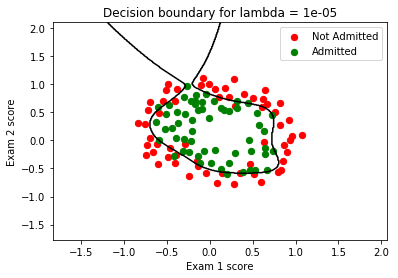
\includegraphics[scale=0.6]{fig4_sk_overfitting.png}
		\caption{Overfitting}
		\label{fig:overfitting}
	\end{figure}
	\begin{figure}
		\centering
		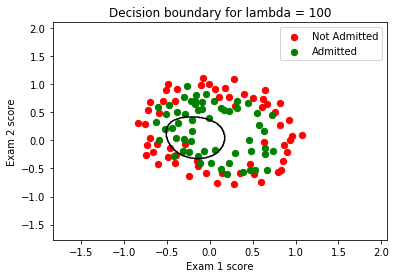
\includegraphics[scale=0.6]{fig4_sk_under-fitting.png}
		\caption{under-fitting}
		\label{fig:under-fitting}
	\end{figure}
\end{itemize}

\paragraph{\textbf{Problem 3 Part C: Fitting regularized logistic regression models (L2 and L1)}}
\begin{itemize}
	\item L2 regularization and log transformation is the best combination for logistic regression model on for this data set for the reason that it has the highest accuracy 0.94140625 on the test set with the best lambda 0.1.
\end{itemize}

\end{document}

